\documentclass[11p]{article}
% Packages
\usepackage{amsmath}
\usepackage{graphicx}
\usepackage{fancyheadings}
\usepackage[swedish, english]{babel}
\usepackage[
    backend=biber,
    style=authoryear-ibid,
    sorting=ynt
]{biblatex}
\usepackage[utf8]{inputenc}
\usepackage[T1]{fontenc}
\usepackage{titlesec}
\usepackage{hyperref}
%Källor
\addbibresource{references.bib}
\graphicspath{ {./images/} }
\usepackage{array}
\usepackage{hhline}

% Lite variabler
\def\email{alvin.hogdal@elev.ga.ntig.se}
\def\foottitle{Gymnasiearbete} % Kanske borde ändras
\def\name{Alvin Högdal}

\title{Gymnasiearbete \\ \small Gymnasiearbete}
\author{\name}
\date{\today}


\begin{document}


% fixar sidfot
    \lfoot{\footnotesize{\name \\ \email}}
    \rfoot{\footnotesize{\today}}
    \lhead{\sc\footnotesize\foottitle}
    \rhead{\nouppercase{\sc\footnotesize\leftmark}}
    \pagestyle{fancy}
    \renewcommand{\headrulewidth}{0.2pt}
    \renewcommand{\footrulewidth}{0.2pt}

% i Sverige har vi normalt inget indrag vid nytt stycke
    \setlength{\parindent}{0pt}
% men däremot lite mellanrum
    \setlength{\parskip}{10pt}
    \begin{otherlanguage}{swedish}


        \begin{titlepage}
            \centering

            % Title and subtitle are enclosed between two rules.
            \rule{\textwidth}{1pt}

            % Title
            \vspace{.7\baselineskip}
            {\huge \textbf{Digitala utvecklingen av datorspeldistribution}}

            % Subtitle
            \vspace*{.5cm}
            {\LARGE Samband mellan tillgänglighet, innovation och påverkan på konsument}

            \rule{\textwidth}{1pt}

            \vspace{1cm}

            % Set this size for the remaining titlepage.
            \large

            % Authors side by side, using two minipages as a trick.
            \begin{minipage}{.5\textwidth}
                \centering
                \name \\
                {\normalsize \url{alvinhogdal@elev.ga.ntig.se}}
            \end{minipage}

            \vspace{3cm}

            % Report logo.
            
\includegraphics[width=0.4\textwidth]{../images/NTI Gymnasiet_Symbol_print_svart.png}

            \vfill

            % University and date information at the bottom of the titlepage.
            NTI Gymnasiet Umeå \\
            Teknikprogrammet\\
            Gymnasiearbete\\
            Datum: \today \\
            Handledare: Jens Andreasson
        \end{titlepage}
        %\maketitle
        %\begin{center}
        %
\includegraphics[width=0.4\textwidth]{../images/NTI Gymnasiet_Symbol_print_svart.png}
        %\end{center}


    \end{otherlanguage}


    \begin{otherlanguage}{english}
        \newpage
\setlength{\parskip}{10pt}

    \section{Abstract}

    The methodology behind distributing video games to consumers has had a strong development during the twenty first century.
    It has changed from buying physical discs to purchasing it digitally and then downloading the video game.
    This study's aim is to figure out what consequences this development has for the consumer.
    The study uses an interview and relevant articles to achieve its aim.
    This study identifies two key indicators in this development.
    The first is the change brought forth by making games more accessible by distributing video games online.
    This means that the consumer has gotten greater access to a greater assortment of video games.
    In turn it has also led to consumers buying products that they potentially do not need.
    It has also led to an obfuscation of the true price for video games since additional content can be sold separately.
    The second is the impact video games have had on society as a place of great innovation.
    The development of video games has had a ripple effect in the technical development of society and smaller actors can distribute their products too.
    \newpage
    \end{otherlanguage}
    \begin{otherlanguage}{swedish}
    \tableofcontents

    \newpage

% i Sverige har vi normalt inget indrag vid nytt stycke\setlength{\parindent}{0pt}
% men däremot lite mellanrum
        \section{Inledning}
        Jag tycker att datorspel är fantastiska.
        Varje datorspel är en unik värld med nya spännande upplevelser, karaktärer, berättelser, historier och så mycket mer.
        Utvecklingen har berört allt från grafik inom datorspel till möjligheter att interagera med datorspel.
        När jag växte upp så hade jag flera möjligheter till att spela datorspel.
        Spelen fanns på cd-skivor som laddades antingen in i datorn eller spelkonsolen.
        Nuförtiden så är de mest digitala kopior av datorspel.
        Att majoriteten av de spel som säljs idag har blivit mer avancerade och komplexa är uppenbart för mig som konsument.
        Möjligheterna inom dessa spelvärldar har ökat i takt med teknikutvecklingen.
        Även möjligheten att ta del av spelutvecklares spel har också ökat exceptionellt på 2000 talet genom att spelen erbjudits till försäljning på fler sätt än i butik.
        \subsection{Syfte \& frågeställning}

    Syftet med undersökningen är att se på de samband som finns mellan den digitala utvecklingen av datorspeldistribution och hur dessa påverkar mig som konsument utifrån dessa två frågor:


    \begin{itemize}

            \item På vilka sätt har spelindustrin utvecklat nya möjligheter att distribuera och sälja digitala datorspelprodukter till konsumenter under 2000-talet?

            \item Hur upplever konsumenter att denna utveckling har påverkat dem?

        \end{itemize}

        \subsubsection{Avgränsningar}
    Detta är ett gymnasiearbete och den digitala spelvärlden är stor.
    Detta arbete utgår från datorspel till konsol eller till dator.
    Studien kommer inte att titta på något specifikt spel.
    Studien tittar på faktorer runt försäljning av tv och datorspel.

        \section{Bakgrund} %källor

    \subsection{ Datorspel i denna studie}
    Att popularitet och därmed den konsumtion av digitala spel som då följer har en stor inverkan på teknikutveckling som en innovations katalysator gör detta ämne både intressant och aktuellt.
    Användandet av ordet datorspel eller termen digitala spel syftar detta i denna studie på kommersiella spel som säljs i syfte att få många spelare.
    Detta inkluderar även de spel som i dagligt tal kallas tv-spel.

    \textcite{ComputerSweden} definition av att datorspel är spel som kräver någon form av dator.
    Detta inkluderar fler saker än bara spel på en dator.
    Denna definition inkluderar även spelkonsoler, arkadspel, vissa brädspel och mer.

        \subsection{Datorspelen som innovations katalysator}
    Funktionerna i ett datorspel och datorns hårdvara är beroende av varandra och kräver kompatibilitet som innebär att både datorer och datorspel utvecklas hand i hand.


    Enligt \textcite{Riksdag} så omsätter datorspel stora belopp och har blivit både så populära och därmed lönsamma att de driver på utvecklingen av hårdvaran.
    Dataspelsbranschen har växt kraftigt i Sverige under senare år, enbart under ett år (2020) så växte den med 40 procent.
    En intressant jämförelse är att dataspelsbranschen är i nu lika i
    storleksordning som den svenska traditionella industrin, av järnmalm och trä.

    En dator bör idag vara en bra speldator för att sälja.
    På ett seminarium som hölls september 2023 i sveriges riksdag lyftes av  Björn Flintberg, forskare på RISE och ansvarig för RISE GameNode, som var inbjuden att tala, att dataspel står för 4 procent av Sveriges totala tjänsteexport och att svenska dataspelsföretag med dotterbolag i utlandet omsätter 58 miljarder per år.
    Han beskriver även dataspelsbranschen som en innovationskatalysator för samhället.

    \setlength{\leftskip}{1cm}
        \("\)Dataspelsbranschen utgör också en innovationskatalysator som har potential för hela Sveriges industri och näringsliv.
        Dataspelbranschen är inte bara i framkant kring nya teknologier, som Artificiell Intelligens och Virtual Reality, utan också en viktig mötesplats mellan kreativ innovation och teknologi, säger Björn Flintberg, forskare på RISE och ansvarig för RISE GameNode.\("\)\parencite{growth}


        \setlength{\leftskip}{0cm}

        \subsection{Datorspelandets påverkan i vardagen}

    Datorspel är något vi alla berörs av idag även om vi inte upplever att vi är aktiva spelare själva.
    Enligt \textcite{Riksdag} så är datorspel inte längre något som kan ses som enskild underhållning utan datorspel är ett aktivt inslag i vårt vardagsliv.
    De komponenter som styr det interaktiva och immersiva är utvecklade av dataspelsbranschen och de i branschen förstår bäst deras användningsområden.
    Idag används denna teknik inom exempelvis arkitektbyråer för att samarbeta med stora projekt på en virtuell plats.
    Många museer erbjuder idag guidning och kunskapsmaterial i interaktiva virtuella miljöer.

    Tekniska museet \parencite{worlds} i Stockholm har följt utvecklingen och skriver på sin webbplats att världarna inom datorspel existerar överallt.
    De finns på bussen, vardagsrummen och kontoren.
    Det finns nästan inga gränser för vart en person kan integrera med digitala spel idag.
    Dessutom så kan de också interagera med andra personer som spelar dessa spel.
    “Datorspel är idag Sveriges genom tiderna största kulturexport och spelen utgör även en grund för Sveriges största subkultur.”

    \setlength{\leftskip}{1cm}
        \("\)Datorspel är idag Sveriges genom tiderna största kulturexport och spelen utgör även en grund för Sveriges största subkultur.\("\)

        \setlength{\leftskip}{0cm}


        \subsection{Försäljning av fysiska datorspel}
        Den fysiska försäljningen av datorspel har minskat till förmån för digital försäljning.
        Detta verifieras på ett flertal trovärdiga internetsidor och av trovärdiga nyhetskällor.
        En källa är webbplatsen Gamereactor som är en webbplats som skriver om datorspel och film.
        Webbplatsen har funnits i Sverige sedan 2002 och skribenten Jonas Mäki är även redaktör på den digitala nyhets plattformen och har funnits med sedan starten.
        I en mycket nyligen publicerad artikel skriver han om spelförsäljningstrenden med nya siffror från i USA.

        \setlength{\leftskip}{1cm}

        \("\)Endast 5\% av den amerikanska spelförsäljningen var fysisk förra året.
        Det verkar som om vi rör oss mot en helt digital framtid i mycket hög hastighet och andelen fysiskt bara minskar\dots
        Vid det här laget var det väldigt många år sedan digital spelförsäljning passerade fysisk sådan, vilket lett till att allt fler titlar endast säljs digitalt, till och med storspel\("\)

        \setlength{\leftskip}{0cm}

        Hans analys i artikeln är följande

        \setlength{\leftskip}{1cm}

        \("\)Detta är naturligtvis en utveckling som tydligt förklarar varför det blir allt svårare att hitta spel i fysiska butiker, och väldigt lite tyder på att denna trend kommer att förändras - snarare tvärtom.\("\)\parencite{amerikanska}

        \setlength{\leftskip}{0cm}

    \subsection{Distribuering via CD rom}
    Fysisk skiva som säljs i butik som innehåller ett datorspel.
    Denna skiva kräver en kompatibel dator med CD-läsare (skivspelare)  eller en kompatibel spelkonsol.
    En svensk definitionen av en CD rom är följande:

    \setlength{\leftskip}{1cm}

    \("\)\("\)Compact disc - read-only memory\("\).
    System för permanent optisk lagring av data på kompaktskivor.
    Skivspelaren ansluts till dator, och skivornas innehåll kan inte ändras eller skrivas över.\("\) \parencite{CD}

    \setlength{\leftskip}{0cm}

    Fysiska dataspelsskivor kan köpas till spelkonsoler som Playstation, Nintendo och Xbox och även vissa spel till PC (persondator)
    Detta sätt att köpa ett spel innebär en engångskostnad för ditt spel.

    \setlength{\leftskip}{1cm}

    \("\)Vid mitten av 1990-talet slog CD-ROM igenom som lagringsmedium, vilket innebar att spelen kunde bli ordentligt mycket mer avancerade och utrymmeskrävande med bland annat fotorealism och filmsekvenser\("\) \parencite{nyckel}

    \setlength{\leftskip}{0cm}

    \subsection{Distribuering via CD-nyckel}
    Cd nyckel är en kod som låser upp ett spel för nedladdning på din dator eller spelkonsol.

    \setlength{\leftskip}{1cm}
    \("\)På Playgames.se säljer vi CD-nycklar som ska aktiveras och laddas ner via exempelvis Steam.
    Du får ingen fysisk produkt med posten.
    Du få en CD-nyckel via e-post och sedan du är redo att spela direkt.
    Håll koll på vårt sortiment eftersom det ständigt kommer nya spel för Mac på Playgames.se.
    Vi säljer spel för Mac via direkt nedladdning.
    Dvs inga fysiska produkter, bara en CD-nyckel som du aktiverar ditt nya Mac spel med och sedan är du redo att spela\("\)\parencite{playgames}

    \setlength{\leftskip}{0cm}
    Detta sätt att köpa ett spel innebär en engångskostnad för ditt spel.

    \subsection{Nedladdningsbart innehåll}
    Nedladdningsbart innehåll eller downloadable content (DLC) är innehåll till ett datorspel som utvecklaren och utgivaren av någon anledning vill hålla separat.
    Det kan vara en uppdatering som ändrar någonting, resurser som används i spelet, kosmetiska ändringar, nya banor eller vapen.
    En DLC kan vara vad som helst.
    Det finns ingen gräns för hur mycket DLC ett datorspel kan ha och det finns inte heller någon gräns för hur mycket det kan kosta.
    Generellt sett så är priset för DLC lägre än vad själva spelet.

    \setlength{\leftskip}{1cm}

    \("\)Nedladdningsbart material kan vara allt från estetiska skillnader till en helt ny berättelse jämförbart med ett expansionspack.
    Ett DLC kan lägga till ett nytt spelsätt, objekt, nivåer, utmaningar, karaktärer eller andra verktyg till ett redan existerande spel.\("\) \parencite{nedladdningsbart}

    \setlength{\leftskip}{0cm}

    \subsection{Battle pass}

    Battle pass är ett system där du köper rätten till att få något innehåll i ett datorspel upplåst, så att du får tillgång till att använda detta i spelet.
    Medan du spelar spelet så låser du upp nya nivåer i battle passet men för att få tillgång till innehållet i den nivån måste du köpa och betala.
    En nivå är som en låda med något innehåll som hör till ett spel.
    Innan en person köper ett battle pass så går det oftast att se hur många nivåer det har och vad som finns i lådorna.
    Generellt sett så är battle pass och dess innehåll endast tillgängligt under en specifik tid.
    Oftast så kan går det också betala för att låsa upp nästa nivå efter köpet av battle passet.

    Att spel säljs med battle pass har blivit vanligare och vad du kommer att behöva betala för en bra spelupplevelse är inte lätt som konsument att veta på förhand.
    Disney med speltillverkaren Gameloft har nu i april månad fått stor kritik över att deras senaste spel Disney speedstorm som går spela på flertalet plattformar har battle pass som du måste köpa för pengar, om du vill vidare i spelet.
    Detta enligt en artikel av \textcite{FZ} skribent på webbplatsen FZ.

    \subsection{Premium valutor}
    En premium valuta inom ett spel är en valuta som spelaren oftast inte kan få genom att spela spelet utan vanligtvis köper för vanliga pengar.
    Kan premiumvaluta fås i spelet så är det oftast i små mängder.
    Det kan ses som en morot för ytterligare större köp och kritik finns mot systemet med premium valutor.
    Om det finns flera olika premium valutor så går det oftast att omvandla dem till andra valutor beroende på.

    \setlength{\leftskip}{1cm}

    \("\)Premium valuta är konceptet att få monetära förmåner när växelkursen mellan två valutor är till en fördel i en valuta.
    Inom spelvärlden sker detta utbyte mellan olika valutor inom ett visst spel eller mellan två olika spel\("\)\parencite{bananatic}

    \setlength{\leftskip}{0cm}

    \subsection{Loot-lådor}

    Loot-lådor är en form av ekonomisk transaktion där du köper en låda som ger dig någonting i ett spel.

    \setlength{\leftskip}{1cm}

    \("\)loot-lådor i data och TV-spel har blivit uppmärksammade den senaste tiden på grund av deras likhet med spel om pengar.En loot-låda kan innehålla någon form av virtuellt föremål som tas fram genom slumpen, till exempel en fotbollsspelare i ett fotbollsspel eller ett nytt sällsynt utseende till en spelkaraktär.\("\)\parencite{sverigesradio}

    \setlength{\leftskip}{0cm}

    Att köpa en lootlåda innebär att du köper någonting fast du vet inte vad det är.
    I en loot låda så finns det oftast väldigt många olika saker med olika chans att få dem.
    Sakerna som en spelare vill ha har oftast väldigt låg chans.
    Låt oss säga att du vill ha en specifik legendarisk sak.
    Det finns en 1\% chans att få en legendarisk sak och det finns 5 olika.
    Alltså en \(1/500\) eller 0,2\% chas att få det du vill.
    Detta system liknar spelmaskiner som finns på casinon med den största skillnaden att du får pengar på casinon och att du får saker inuti spelet från loot-lådorna.


    \setlength{\leftskip}{1cm}

    \("\)Lootlådor är en sorts hemlig låda i tv-spel som går att köpa för riktiga pengar.
    I den får spelaren slumpmässiga föremål och figurer som går att använda i spelvärlden, inte helt olikt gamla tiders hockeykort.
    Sveriges konsumenter är kritiska, och liknar det vid lotterier.
    - Det är en väldigt aggressiv marknadsföring som ofta gränsar till att vara direkt vilseledande.
    Man använder sig av påhittade valutor som exempelvis diamanter och poäng i stället för att redovisa vad det faktiskt kostar, säger Sinan Akdag, digital expert på Sveriges konsumenter.\("\)\parencite{loot}

    \setlength{\leftskip}{0cm}



    \subsection{Vad kan detta nya sätt att konsumera digitala produkter innebära för mig som konsument?}
    Att äga sitt fysiska spel innebär att du med en kompatibel enhet alltid kan spela ditt spel.
    Det vill säga så länge din digitala skiva håller eller din digitala enhet.
    \textcite{support} som är ägare av företaget Xbox listar följande fördelar för dig som konsument med att konsumera digitala spelprodukter.
    \begin{itemize}
        \item \("\)Med digitala spel är det enkelt att gå från ett spel till ett annat utan att behöva byta skiva – eller hitta skivan om du har glömt var du har den.\("\)
        \item \("\)Dina spel måste laddas ned till din enhet oberoende av om de är fysiska eller digitala, och de tar upp lika mycket utrymme. Men digitala spel ger dig mycket mer flexibilitet, som fjärrinstallation och förinläsning innan spelen startar.\("\)
        \item \("\)Digitala spel kan delas med alla som loggar in på din hemma-Xbox. Det inkluderar spel som erbjuds via en Xbox Game Pass-prenumeration. Och du kan spela digitala spel som du äger var du än är inloggad. Ingen skiva krävs.\("\)
        \item \("\)Genom att ge spel i present direkt från Microsoft Store till vänner och familj får du ett jättebra (och superenkelt) sätt att visa hur generös du är.\("\)
    \end{itemize}


    \subsection{Identifierbara digitala faror för mig som konsument}

    Det finns många kritiska röster mot spelbolagens sätt att tjäna pengar genom sina nya distributionssätt av spel eller innehåll till spel.
    Flera studier har gjorts och flera europeiska länder har tillsammans krävt förbättringar kring konsumentskydd inom detta område.
    Det finns tydliga indikationer på casino liknande försäljningsmetoder, som återfinns i spelen, kan leda till ekonomiskt spelmissbruk.
    Det finns en norsk studie \("\)Insert Coin\("\) från 2022 som blivit uppmärksammad stort som handlar om de casino liknande sätt spelindustrin utnyttjar konsumenter.
    Detta har lett till regeringskrav att se över regleringen runt spelindustrins försäljningsmetoder.

    \setlength{\leftskip}{1cm}

    \("\)Tillsammans med 19 andra europeiska konsumentorganisationer kräver Sveriges Konsumenter förbättringar av konsumentskyddet för europeiska gamers, särskilt för barn.
    Bakgrunden är en ny rapport där den norska konsumentorganisationen Forbrukerrådet har granskat spelindustrins oschyssta affärsmetoder.
    \begin{itemize}
        \item Påhittade valutor som döljer vad köpen i spelen verkligen kostar.
        \item Svårtydda och ibland vilseledande beskrivningar av sannolikheten att vinna.
        \item Speldesign som medvetet utnyttjar psykologiska sårbarheter och manipulerar spelare att spendera mer pengar.
        \item Aggressiva marknadsföringsmetoder, i vissa fall riktade mot barn\("\)\parencite{insertcoin}
    \end{itemize}
    \setlength{\leftskip}{0cm}

        \section{Metod}

    För att belysa på vilket sätt spelindustrin utvecklat nya sätt att distribuera och sälja spel, gjordes en sammanställning i studiens bakgrundsdel. Studien tittar på samband utifrån de olika sätt som spel distribueras idag, vid en försäljning, till sina produktsystem, dator eller konsol.

    Metoden som valdes till studien är kvalitativ. Den kvalitativa metoden ansågs som bäst utifrån syftet med studien. Studiens område handlade om att ge en bättre förståelse för vad konsumenter upplever,  och även varför de tycker på det sättet.

    Tre intervjuer gjordes med datorspelkonsumenter utifrån ett intervjuformulär. Dessa genomfördes som telefonintervjuer. Intervjuerna spelades in för att sedan transkriberats och analyseras. Det relevantaste innehållet i intervjupersonernas svar har sammanställts i resultatet.  Intervjuerna finns i sin helhet som bilagor. De intervjuade personerna benämns som Gamer 1, Gamer 2, och Gamer 3.  Intervjufrågorna som ställdes finns med som bilagor.


    Intervjuerna genomfördes för att i den kvalitativa metod som används i denna studie, låta några dela med sig av personliga åsikter och erfarenheter. Val av intervjumetod har utgått från en metodguide för inkluderande intervjuer. En semistrukturerad intervju ansågs som bäst för att uppfylla syftet med studien.

        \("\)I en semistrukturerad intervju utgår du ifrån ett antal övergripande frågeområden och anpassar fördjupningsfrågorna efter hand.\("\) \parencite{Metodguide}

    Urvalet för denna studie, då det är ett gymnasiearbete, begränsades till antalet intervjupersoner till tre.
    En viktig faktor i urvalet var att välja ut några personer i ålder så att de personerna varit med om senaste årens utveckling av konsumtion och distribution av datorspel.
    Att intervjupersonen identifierade sig själv som en gamer var även en viktig faktor för studiens resultat och för urvalet att personerna representerar en uppskattningsvis genomsnittlig spelare.
    Eftersom män enligt \textcite{folkhalsa} är mer frekventa spelare än kvinnor, så valdes tre män.
    Männen som valdes var födda tre olika decennier.
    Anledningen till det åldersurvalet var för att eventuellt få ökade möjligheter till en bredare bild i den beskrivna upplevelsen utifrån frågeställningen.
    Intervjupersonerna var vid intervjutillfället 51, 43 respektive 28 år gamla.

    Intervjufrågorna har valts för att tydliggöra konsumentens upplevelse av den digitala utvecklingen i dataspel distribution.
    För att vara relevant för studien är det viktigt att den intervjuade personen hade egna erfarenheter inom detta område.

    Den första frågan syftar till att säkerställa om den intervjuade personen ser sig själv som en aktiv spelare av datorspel, en gamer.
    Den andra frågan syftar till att säkerställa om personen även varit gamer över en längre tidsperiod.
    Fråga tre och fyra handlar om intervjupersonens förmåga att identifiera eventuella förändringar i konsumtionsmönster utifrån det digitala sättet att få sitt datorspel levererat och vad intervjupersonen tycker om att inte äga fysisk produkt.

    Fråga 5 med följdfrågor syftar till att inklusionskriterierna i studien är uppfyllda. För att få så relevanta resultat som möjligt är det viktigt att säkerhetsställa intervjupersonens kunskap om nya distributionssätt.
    Frågorna 6 och 7 syftar till att se om intervjupersonen kan identifiera upplevelsen av denna digitaliserade utveckling kring konsumtion datorspel i  positiva respektive negativa konsekvenser, utifrån syftet med studien.

    Intervjuerna bearbetades utifrån en tematisk analys perspektiv. Denna metod valdes eftersom det ansågs vara en bra metod för att identifiera gemensamma nämnare i intervjuer och sedan sammanställa dem. Detta gjordes utifrån en induktiv analysmetod vilket betyder att låta sig inspireras av de teman man hittar i intervjumaterialet och dra slutsatser därifrån.

    Detta genomfördes genom att först transkribera och sedan noga läsa igenom intervjuerna. Därefter markerades stycken som ansågs relevanta för studien med överstrykningspenna. Små noteringar gjordes i marginalen, det som enligt den tematiska analysmetoden benämns som kodning, för att se vilka teman som framkom. Enligt denna metod är det därmed  dessa teman som bör belysas i resultatet, utifrån det transkriberade intervjumaterialet, detta återfinns därmed i resultatet.

    Kunskapen om hur man genomför en tematisk analys hämtades från en föreläsning av Olov Aronsson. Forskare, filosofie doktor och grundare till Kvantila.\parencite{tematisk}


    \section{Resultat}

    Studien syftar till att se på samband mellan den digitala utvecklingen av datorspelsdistribution och hur det påverkat konsumenten. I bakgrunden till studien belyses aktuella faktorer runt konsumtion och distribution.  En bärande faktor i denna studie är att datorspelsindustrin kan ses som en innovations katalysator i samhället i stort. Detta utifrån både i hur spelindustrin genererat ökade intäkter i samhället i stort och hur skapade innovationer idag används på flertalet ställen i samhället.

    Utifrån de intervjuade konsumenternas upplevelse kan vi se flertalet gemensamma nämnare i hur de upplever denna utveckling som enskild konsument. Dessa gemensamma nämnare kommer nedan att presenteras. Studiens sammanfattade resultat tydliggörs under rubriken “Den digitala tidsåldern”

    \subsection{Fler aktörer ökat utbud}
    Intervjupersonerna använder termen indiespel när de beskriver enskilda individer, eller små aktörer som utvecklat spel utan någon stor speltillverkare bakom sig. Två av de intervjuade personerna uttrycker en positiv utveckling där de mindre datorspelsutvecklarna kan få ut sin produkt på marknaden och att de därmed kan ta del av den.

    \setlength{\leftskip}{1cm}

    “Så det är ju det ena och det andra som jag personligen tycker är extremt positivt är ju att de här mindre spelföretagen som speltillverkare får ju ut sin produkt.
    Jag menar indiespel är väl ett typexempel på det på nåt sätt.  Alltså små, små, små spelföretag som kanske har en helt genial spelidé. Som kanske har ett litet spel. Det kanske inte ens är så speciellt grafiktbaserat. Det kanske inte är som så, utan det är bara en sjukt bra spelidé. Och sen så är det inte superdypt. Och man kom ju åt det. För de fanns ju inte få tag i förut

    \dots

    Att du kan ju hitta mycket mer innehåll. Och framförallt som sagt du kommer inte bara åt de här stora AAA titlarna. Utan man kommer åt mycket annat innehåll. Vilket är ju fantastiskt. Och den typen av spel tilltalar ju mig mycket mer. Rent generellt. Så det är ju väldigt positivt.” Gamer 1


    \setlength{\leftskip}{0cm}

    Gamer 1 jämför detta med utvecklingen av musik och streamingtjänster som Spotify idag och jämför indiespel  på samma sätt som om man tittar på musik


    \setlength{\leftskip}{1cm}
    “Skulle man köpa en hårdrocksskiva 1986.
    Så gick man på musikaffären. Och så tittade man på de 47 olika banden som fanns som de hade på en välsorterad butik. Och så var det något att välja något av dem. Nu finns det ju 4900 band.” Gamer 1


    \setlength{\leftskip}{0cm}
    Även gamer 3 lyfter detta tydligt:

    \setlength{\leftskip}{1cm}
    “Framförallt att det är bra för de mindre spelutvecklarna att kunna hitta en plattform. Det har ju ändå blivit några sådana fall.
    Det har varit svårare för dem tidigare. Det har varit mer de stora drakarnas marknad. Som har fått göra o sälja sina spel i spelbutiken.
    Men nu går jag verkligen för alla. Även för de minsta, att få ett genomslag  bara man hamnat på en topplista och lyckats bli känd för att folk gillar ens spel.” Gamer 3


    \setlength{\leftskip}{0cm}
    Av citaten så framgår det väldigt tydligt att mindre företag kan få ut sin produkt på marknaden och nå konsumenter. Det brukade vara “de stora drakarnas marknad” där endast etablerade företag existerade. Det fanns endast en begränsad mängd utrymme på hyllorna och det fanns endast plats för datorspel som garanterat säljer. Med den tekniska utvecklingen så finns det ingen fysisk begränsning av utbudet. Ett datorspel måste inte sälja stort för att finnas på marknaden. Det digitala sättet att leverera datorspel möjliggör existensen av de mindre aktörerna.


   \subsection{Att handla i en butik där varan inte kan ta slut }

    Gemensamt för alla intervjupersoner är att de beskriver mycket positiva sidor av den digitala distributionensutvecklingen i sin roll konsument.


    \setlength{\leftskip}{1cm}

    “Det blir mycket lättare att köpa spel och det blir att man ser alla spelen. Man måste inte resa till en butik för att se hur många som finns och vad som finns hemma framförallt. Nu tar ju aldrig spel slut så det är aldrig slut på lagren.“ Gamer 2

    “Det är ju extremt tillgängligt. Jag har ju chans att\dots Man kan ju prova på väldigt, väldigt mycket. Det är ju lätt. Väldigt många spel kommer ju med speldemos som man kan prova på i förväg. På väldigt många. Och testa. Verkar det här vara någonting för mig? Men det är ju extremt tillgängligt. Jag kan komma på klockan 11 på kvällen att jädransch i min lilla låda. Det här spelet såg ju sjukt kul ut. Det här vill jag provspela. Och så kan jag spela det klockan 10 över 11 med lite tur.“ Gamer 1

    “Då man ändå oftast köper och visar sina spel på Steam , såsom jag som har bott utomlands har ändå kunnat ha tillgång till exakt samma spel på en annan dator.Det enda som har varit skillnaden har ju varit att man har behövt installera dem om det inte har varit installerat på en dator, men går man på ett spelcafé typ och hyr en dator så finns ju oftast ändå de största mainstream-spelen installerade.“ Gamer 3

    \setlength{\leftskip}{0cm}
    Det positiva som går att identifiera i intervjuerna är att bara i princip på ett klick kunna få tillgång till spelvärlden. Det kan vara allt från information om datorspel, hitta demo av något datorspel, se livestreamade datorspel, få reklam och reapriser om datorspel, läsa andras recensioner, få tydlig info om hur svårt datorspelet är till att kunna ladda hem datorspelet vilken tid på dygnet som helst.

    \setlength{\leftskip}{1cm}
    “Ja, det är ju att det\dots Det sparar ju mig en fruktansvärd massa tid. Att bara äta. Jag behöver inte planera att fara och köpa det någonstans överhuvudtaget. Jag bara. Man tankar bara ner det när man är sugen. Och då har man oftast supporten på samma ställe. För hur man shoppar och sådär. Det är ju bekvämt. Bekvämt som rackarns” Gamer 2

    \setlength{\leftskip}{0cm}
    Som Gamer 2 här beskriver det går att tolka som att han nästan ser det som att vara på en positiv trevlig restaurang när han använder termen som “äta direkt”, “ när man är sugen”.

    
    \subsection{Att köpa, men inte få en vara!}
    Spelindustrin har utvecklats till att du idag köper något annat än tidigare. Intervjupersonerna ser på detta i lite olika vinklar. Du äger inte längre den vara som du köpt fysiskt, kan inte sälja den vidare utan du har mer köpt tillgång till en tjänst idag.

    \setlength{\leftskip}{1cm}
    “De säljer ju i princip en rättighet att spela spelet men du äger ju ingenting.
    Och du vet ju knappt nu för tiden hur länge du får kvar den där äganderätten.
    Eller liksom att du får spela det, därför att helt plötsligt så läggs ju spel ner.
    Att det är spel som kräver en onlineaktivitet eller du måste ha en server
    koppling och så läggs servern ner och så går ju spelet inte att spela
    överhuvudtaget. Och så har det ju aldrig varit
    Men just att det att fysiskt inte äga det påverkar mig personligen  inte negativt alls. Så jag tycker att det inte är ett problem överhuvudtaget. Men jag förstår att det är många som tycker det.
    Att man inte äger, äger den vara man har köpt på något sätt. Man köper inte en vara längre utan man köper mer en tjänst.Det förstår jag att många tycker  är negativt.”  Gamer 1

    Vad tycker du om utvecklingen att inte äga en fysisk produkt?

    \setlength{\leftskip}{2cm}
    “I början var det inte ett så stort problem men man började tänka på det mer och mer eftersom att det börjar, har ju utvecklats till det att ja men, folk köper online spel och sånt där och har inte rättighet att behålla det.

    \dots

    Nu sitter man ju bara och hoppas på att man inte ska bli kickad från en hel, typ rockstar game deras\dots vad heter den nu,  social club.
    Den kan man ju blir kickad av om du missköter liksom.“ Gamer 2

    \setlength{\leftskip}{0cm}
    Att den digitala förändring av försäljningen som ger andra förutsättningar för dig som konsument än tidigare, är något Microsoft listar som positiva fördelar för dig som konsument på sin webbplats, vilket belyses under bakgrund i denna studie. Där kan man utläsa att det är positivt att du kan spela digitala spel som du äger var du än är inloggad. Ingen skiva krävs,  Med digitala spel är det enkelt att gå från ett spel till ett annat utan att behöva byta skiva – eller hitta skivan om du har glömt var du har den, menar Microsoft.
    Ser man på  denna information i deras försäljningsargument till dig som konsument kan man utifrån denna studie dra slutsatsen att de syftar till att de säljer en likadan vara som tidigare, men att intervjupersonerna är av en annan uppfattning. De köper en helt annan produkt i dag som kommer med helt nya användarvillkor än tidigare.

    \subsection{Köpa mer än planerat}

    Utifrån att tillgängligheten till köp ökat så identifierar intervjupersonerna  att deras köpbeteenden har ändrats. De beskriver hur de tidigare planerade sitt köp, åkte till spelbutiken och köpte sitt spel. Men nu så klickar de hem intressanta spel. Man kan utifrån intervjuerna se att det finns en tendens till att köpa mer än planerat.

    \setlength{\leftskip}{1cm}

    “Förr i tiden när man faktiskt var tvungen att fara och köpa fysiskt spel, att köpa en diskett en gång i tiden, men sedan på cd-skivor eller DVD och så vidare, så hade man ju en plan

    \dots

    jag har aldrig farit för att titta i affären, undra vad de har för spel? Undrat finns det någonting jag skulle vilja ha. Jag har ju alltid när jag köpt spel, då har man farit för att köpa ett specifikt spel, åt sig själv i alla fall.

    \dots

    Nu med det digitala blir det mycket mer impulsköp av spel. Att ooo det här se ju spännande ut

    \dots

    det här kanske jag ska prova. och så spontanköpte man det”  Gamer 1

    \setlength{\leftskip}{0cm}
    Utifrån intervjun med Gamer 2 så kan man dra slutsatsen att även han inte planerar sina inköp på samma sätt som tidigare. Han svarar på frågan om det digitala sättet att leverera spel har påverkat hur du konsumerar spel och i så fall hur?

    \setlength{\leftskip}{1cm}
    “Ja, ju mer du kan köpa online och ju billigare det blir, vissa spel alltså. Så blir det ju enklare att köpa över internet och tanka ner på att installera det.” Gamer 2

    \setlength{\leftskip}{0cm}
    Gamer 3 är inne på att det kan bli en överkonsumtion när han får frågan om han kan se negativa konsekvenser för dig som konsument att spel levereras digitalt.

    \setlength{\leftskip}{1cm}
    “Ja, det blir som aldrig bra med en överkonsumtion eller det blir för  mycket tillgängligt. Det är klart att det kan finnas något negativt med det.” Gamer 3


    \setlength{\leftskip}{0cm}
    Detta bekräftas tydligt av Gamer 1 som ger en personlig bild av sig själv som impulsshoppare.

    \setlength{\leftskip}{1cm}
    “Det som möjligen för mig är negativt är väl att man spontant shoppar lite för mycket spel som man nästan inte spelar i slutändan. För man bara ooo det här såg ju lite kul ut. Och så har man råkat köpa lite alltihop. För att det går så fort. Det är ju så mycket impulsshopping. Jag är en ganska effektiv impulshoppare. Så det är väl inte helt positivt för mig. Då är det bättre om jag var tvungen att tänka en stund. Ibland.” Gamer 1

    \setlength{\leftskip}{0cm}
    Det vi vet är att dataspelsbranschen ökat sina intäkter kraftigt och att dessa intäkter kommer från konsumentled. Under rubriken bakgrund har denna studie beskrivit dataspelsbranschen tillväxt och att dataspelsbranschen har växt kraftigt i Sverige under senare år. Under året 2020 så växte den med hela 40 procent.
    Att den digitala datorspeldistributions utvecklingen gett ökade möjligheter eller risker till ett impulsivt handlande påvisas av intervjupersonernas berättelser.

    Att detta förändrade distributionssätt i konsumentled lett till mer inköp än planerat, är en möjlig slutsats att dra utifrån de intervjuade personerna. Att detta i sin tur bidragit till den ekonomiska utvecklingen för spelindustrin, är en sannolik slutsats man skulle kunna dra utifrån detta.

    \subsection{Spelbolagens nya distrubutonssätt är begränsande för återförsäljning och ägande  }
    Alla intervjupersoner visar utifrån intervjufrågorna som rör distributionssätt som behandlas i studien, en genomgående hög kännedom.   På frågorna om CD-nycklar för nedladdning, Nedladdningsbart innehåll, Battle pass, Premium Valutor, Loot lådor och Steam visar de medvetenhet om spelindustrins nya distributionsvägar. Det går också utifrån intervjuerna att identifiera hur de till viss del genomskådar spelindustrins begränsningar till återförsäljning och de försäljningsmekanismer bolagen skapat för att generera mer inkomster till bolagen.
    Nedan ges några belysande exempel:

    CD-nycklar

    \setlength{\leftskip}{1cm}
    “Att du köpte ut spel fysiskt men sen så var det fortfarande så att du var tvungen att ha en licens för att du bara skulle kunna ha en användare. Det är ju till viss del för att begränsa då återförsäljningsmöjligheterna eller som att du skulle kunna sälja det vidare.” Gamer 1

    \setlength{\leftskip}{0cm}
    Lottlådor.

    \setlength{\leftskip}{1cm}
    “Ja, det är ju som att spela på ett casino ungefär. Man betalar pengar och så. Oftast betalar man pengar men kan även få det som dropp, alltså att man får det gratis. Men det är ju ofta att man får det gratis för att man ska lockas in för att köpa senare i spelet och så kan man väl få olika grejer. Antingen göra spelupplevelsen. Som är starkare för ens karaktär eller visuellt.” Gamer3

    \setlength{\leftskip}{0cm}
    Battle Pass.

    \setlength{\leftskip}{1cm}
    “Battle Pass är ju då att du har köpt ett spel. Och släpper dem som små uppgraderingar till spelet som du kan köpa. För att sen spela dig till det efterhand, vilket är ganska fucked up. Så Battle Pass är väl som en ny säsong i ett spel kan man säga.” Gamer 2


    \setlength{\leftskip}{0cm}

    Utifrån intervjupersonernas svar kan vi se en koppling till att de nya försäljnings och distribueringsmetoderna av datorspel är en aktuell fråga.  Bakgrunden till denna studie beskriver att europeiska konsumentorganisationer kräver förbättringar av konsumentskyddet för europeiska gamers utifrån spelindustrins oschyssta affärsmetoder. Att påhittade valutor döljer vad köpen i spelen verkligen kostar. Speldesign som medvetet utnyttjar psykologiska sårbarheter och manipulerar spelare att spendera mer pengar och aggressiva marknadsföringsmetoder. Detta är faktorer som gör att du blir sårbar som konsument och faktorer som sannolikt bidragit till den ekonomiska utveckling spelbolagen har haft.

    \subsection{Den digitala tidsåldern}
    Analysen av resultatet visar att det sannolikt har varit bidragande till den innovativa utvecklingen med att fler aktörer, som Gamer 1 uttrycker det “ inte bara stora drakar” har fått komma till fram till konsument. Det nämns som positivt för konsumenter i intervjuerna, med det ökade utbudet av små aktörer och att detta tilltalar intervjupersonerna.

    Fler idéer i både försäljningsled och fler idéer i produktled har lett till ökat utbud och detta har samtaget med ökat intresse från konsument bidragit till den innovativa utveckling vi ser idag. Spelbranschen har blivit som ett genererande hjul som snurrar snabbt där spelbranschen både är och har varit drivande.

    Genom de nya möjligheter, i den digitala världen som skapats och som har haft en tydlig utveckling under 2000-talet, har det skapats helt nya både konsumtions- och distributionsmöjligheter.

    Det finns idag digitala plattformar att få mötas på där konsumenter och utvecklare idag möts. Detta har då skapat stora möjligheter till utveckling genom tillgänglighet för båda sidor, både från konsumenter och spelutvecklare.

    Konsumenten har fått betydande större tillgänglighet till att ta del av  utbudet.
    Produktutvecklaren har i sin tur fått betydande större möjlighet att nå ut till konsument

    Detta kan beskrivas som i följande bild.
    \begin{figure}[!h]

        \center
        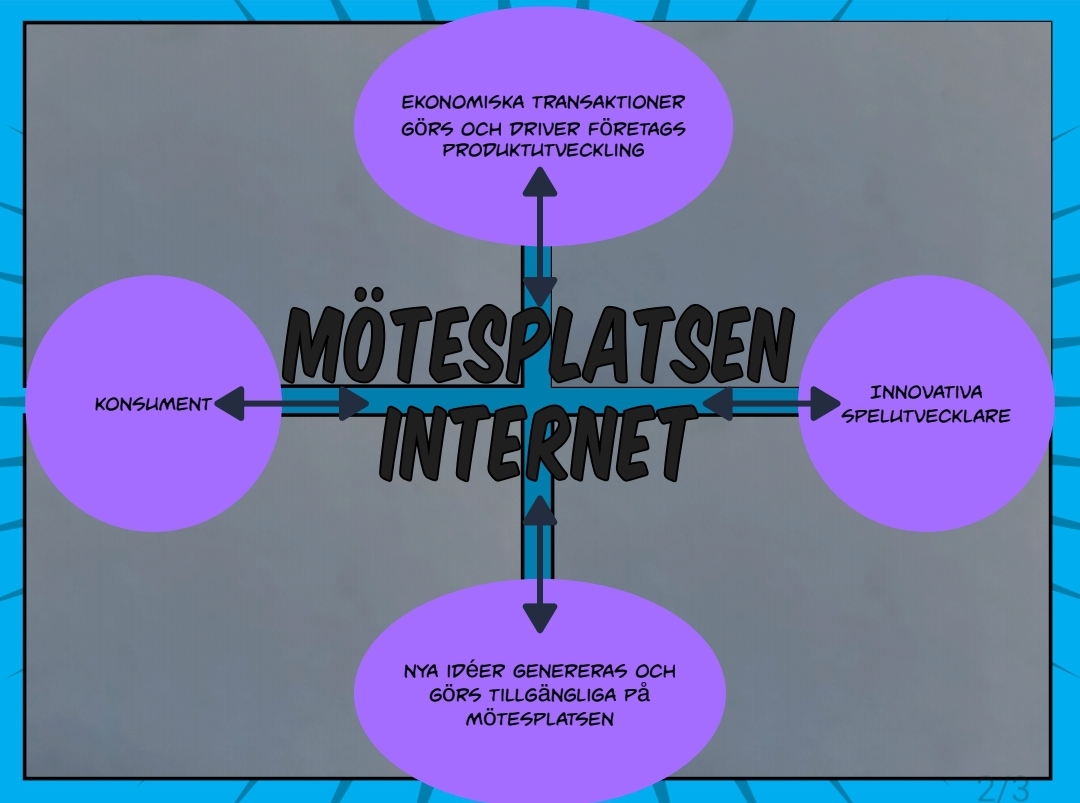
\includegraphics[width=0.8\textwidth]{../images/inte_episk_bild}
        \caption{Bild på konsumtionscirkel}

        \label{bild:cirkulär}
    \end{figure}

    \begin{figure}[!h]
    Det finns som studien visar många olika aspekter på de samband man kan se mellan den digitala datorspeldistributionens och påverkan för konsument. Studien visar på samband mellan den enskilda konsumenten som idag inte längre äger sin fysiska produkt, som idag köper en annan vara än tidigare och den innovationsutveckling som detta genererat i samhället som stort.
    \end{figure}
\newpage
    \section{Diskussion}

        Studien visar på att utvecklingen av sätt att distribuera spel förändrats markant under 2000 talet.
        Att spelindustrin hittat flera olika vägar eller sätt att distribuera spelproduketer och att det gått från ett fysiskt fast köp av en spelprodukt till att du digitalt köper delar, prenumerationer, uppdateringar och kosmetiskt innehåll.

        Detta innebär för konsumenten att det är svårt att veta på förhand vad du kommer att spendera på ett spel.
        Detta har fått konsumentorganisationer runt om i Europa att reagera och kräva förbättringar av konsumentskyddet.

        Att som enskild konsument råka köpa fler spelprodukter än vad du planerat och tänkt från början bekräftas i intervjun med gamern.
        Gamer 1 beskriver sin impulsshopping av spel som det enda problemet han ser med den digitala utvecklingen.

        Alla intervjuade delar ändå i stort sett bilden med Microsoft i att de  upplever att utvecklingen i det mesta är positiv. Datorspel har blivit extremt mer tillgängliga att få tag i. Urvalet av spel som finns att köpa har ökat markant. Innovationerna har ökat, utbudet ökat och tillgängligheten blivit helt annat.ö

        De lyfter möjligheten för mindre speltillverkare att komma ut med sin produkt. Eftersom urvalet av spel inte begränsas av vad som generellt kan säljas på en hylla i affären utan vad som säljer tillräckligt bra för att få tillbaka produktionskostnaderna från enskilda konsumenter i olika länder. Nu kan vem som helst med kunskap om att utveckla ett datorspel, med en bra idé, skapa ett dataspel och göra det tillgängligt för världens konsumenter.

        Dataspel är en stark tillväxtbransch, omsätter miljardbelopp och att detta är en pågående innovations katalysator i samhället kan ses som en mycket intressant faktor. Samtidigt med spelbolagens ökade möjligheter till inkomster har detta genererat något som definitivt har potential för hela Sveriges industri och näringsliv. Innovativ teknik som är här för att stanna och för att hela tiden vidareutvecklas.

        Konsumentskyddet bör stärkas så att den enskilde inte luras till köp utan att konsumenten tydligt vet vad den köper och vad det kostar.
        Man skulle ändå sammanfattningsvis kunna säga att spelbolagens intresse i att skapa mer inkomster till sig har skapat värde för en hel mänsklighet, konsumtionssamhället ur sina bästa aspekter.

        Att detta är en bransch i ständig utveckling gör detta mycket intressant att fortsätta följa. En gamer idag är inte någon som sitter i sin ensamhet och spelar nördiga spel. En gamer är idag en del av den nya innovationen.


    \setlength{\leftskip}{0cm}

        \newpage
        \section{Referenser}
        \printbibliography[heading=none]

        \newpage
        \section{Bilagor}

        \subsection{Bilaga 1}
        Intervju - Gamer 1

        Mitt gymnasiearbete handlar om att undersöka det samband som finns mellan den digitala utvecklingen av spel distribution och hur detta påverkar konsumenter utifrån rollen som konsument av datorspel.

        Då undrar jag, kan du identifiera dig med ordet gamer i bemärkelsen att du är en konsument av datorspel?


        \setlength{\leftskip}{1cm}

        Ja, det kan jag göra.

        \setlength{\leftskip}{0cm}
        Har du varit konsument av datorspel under perioden då spelförsäljningen har övergått till mer och mer digitala sätt att leverera spel.


        \setlength{\leftskip}{1cm}

        Ja, jag har ju varit en spelkonsument sedan 80-talet så absolut.

        \setlength{\leftskip}{0cm}
        Har det digitala sättet att leverera spel påverkat hur du konsumerar spel och I så fall, hur?


        \setlength{\leftskip}{1cm}

        Ja, det har det ju absolut gjort.
        Förr i tiden när man faktiskt var tvungen att köpa spel, att köpa en diskett en gång i tiden, men sedan på cd-skivor eller DVD och så vidare, så hade man ju en plan.
        Man for ju oftast inte för att, jag har aldrig farit för att titta i affären och undra vad de har för spel, undra varför finns det någonting jag skulle vilja ha. Jag gör alltid det när jag har köpt spel, då har man farit för att köpa ett specifikt spel åt sig själv i alla fall. Möjligen som en present när man har gett bort saker så kanske man har gjort annorlunda.
        Men när man ska köpa åt sig själv så har man ju farit för att köpa något specifikt till sig själv.

        Nu med det digitala så blir det mycket mer impulsköp av spel. Ooo Det här ser ju spännande ut.
        Man ser liksom att det är en reklam på det. Eller någon som man klickar runt på  Youtube eller Twitch. Det här såg ju spännande ut, det här kanske jag ska prova. Och så spontan köpande.
        Så absolut, det är inte lika planerat spel shoppande nu för tiden utan det är mycket mer impulsstyrd. Det är mycket mer tillgängligt.


        \setlength{\leftskip}{0cm}
        Vad tycker du om denna utveckling att inte äga en fysisk kopia av ett spel?

        \setlength{\leftskip}{1cm}

        Ja, det där är ju en otroligt intressant fråga.
        Framförallt med tanke på att fler och fler plattformar börjar ju dessutom, säljer de inte ens äganderätten till spelet.
        De säljer ju i princip en rättighet att spela spelet men du äger ju ingenting. Ää Och du vet ju knappt nu för tiden hur länge du får kvar den där äganderätten.
        Eller liksom att du får ens få spel, därför att helt plötsligt så läggs ju spel ner.

        Att det är spel som kräver en onlineaktivitet eller du måste ha en server koppling eller så läggs ju en server ner och så går inget spel att spela överhuvudtaget. Och så har det ju aldrig varit.
        Så var det inte förut. Du har ju inte, förr så kunde du ju ändå köpa ett spel, du kunde spela det och sen kunde du ju faktiskt sälja det vidare.

        Då hade du ju en fysisk kopia och det gick liksom generellt i alla fall. Att det faktiskt fanns ett andrahandsvärde i spel, det har ju helt försvunnit.
        Det går ju inte med möjligen vissa unika undantag. Men så går det ju inte att sälja sitt spel vidare generellt.
        Och sen om det då är positivt eller negativt, hur det påverkar mig.

        Personligen så har jag aldrig sålt ett spel vidare på det sättet.
        När man har spelat klart det så är man ju så nöjd och belåten. Och sen så faller de ju lite i en glömska.

        Jag är ju inte en sån som när jag spelar ett spel så att sen tio år senare eller fem år senare kommer jag och bara ooo det här skulle jag plocka upp igen. Jag funkar inte på det sättet. Då söker jag in någonting nytt. Jag kan absolut spela omspel, det finns spel som har omspelsvärde.
        Men just att det fysiskt inte ägare påverkar mig personligen, inte negativt.

        Så jag tycker att det inte är ett problem överhuvudtaget. Men jag förstår att det är många som tycker det.
        Att man inte äger den vara man har köpt på något sätt. Du förstår att många tycker det är negativt. Men personligen så är det inte alldeles något problem.
        Det påverkar inte det sättet som jag använder spel på. Det påverkar inte det på något sätt för mig.


        \setlength{\leftskip}{0cm}
        Jag har några termer och jag undrar om du vet om vad det är och samt vad dom är.
        Cd-nyckel för nedladdning.


        \setlength{\leftskip}{1cm}

        Vill jag bara svara om jag förstår vad det betyder eller vill jag förklara vad det betyder? Jag vet vad det är för någonting.

        \setlength{\leftskip}{0cm}
        Du kan nästan bara enkelt förklara om du förstår vad det betyder.

        \setlength{\leftskip}{1cm}

        Ja men jag förstår absolut vad du menar. Vad det innebär.
        Det är ju helt enkelt en digital produktnyckel för att låsa upp en digital produkt. Det finns ju även en CD-nyckel. Det fanns ju även på den fysiska tiden. Att du köpte ut spel fysiskt.
        Men sen så var det fortfarande så att du var tvungen att ha en licens för att du bara skulle kunna ha en användare. Det är ju till viss del för att begränsa på försäljning möjligheterna. Eller att kunna sälja det vidare. Eller att låsa upp en produkt.


        \setlength{\leftskip}{0cm}
        Nedladdningsbart innehåll. Eller mer känt som downloadable content.

        \setlength{\leftskip}{1cm}

        Vad sa du? Nedladdningsbart innehåll. Eller ja DLC okej. Jag slutar där. Det är ju extra material om man säger så.
        Tilläggsmaterial som släpps till spel. För att du släpper ett spel som innehåller\dots Om du jämför med en bok så släpper du en bok som innehåller tio kapitel.
        Men sen kan du köpa till kapitel 11, 12 och 13 om du är nyfiken. Och vill veta vad som faktiskt inte hände. Men det är ju liksom så att det är extra material som du kan betala för då. Framförallt. Och ladda ner. Alltså tilläggsinnehåll i spelet.


        \setlength{\leftskip}{0cm}
        Battle Pass.

        \setlength{\leftskip}{1cm}

        Battle Pass. Ja, det är ju Blizzards version av\dots Det får vi ändå kalla för en prenumeration. På något sätt.
        På en online tjänst egentligen. Sen var det så extremt länge sedan jag har haft Battle Pass en gång i tiden. Men det har inte varit så länge sedan jag har använt det.
        Så om det har förändrats över tid så är det typ samma. Men i grund så är det väl en förmån och klassare som en prenumeration på en online tjänst egentligen. För att komma åt deras katalog.


        \setlength{\leftskip}{0cm}
        Premium-valutor.

        \setlength{\leftskip}{1cm}
        Förlåt, nu hörde jag inte vad du sa.


        \setlength{\leftskip}{0cm}
        Premium-valutor.

        \setlength{\leftskip}{1cm}

        Alltså pengar i spel. Antaget du pratar om nu.


        \setlength{\leftskip}{0cm}
        Ja.

        \setlength{\leftskip}{1cm}

        Det vill säga att det finns ju interna valutor i spel. Finns det ju pengar. Du kan ju ha interna shoppar. Och de interna valutorna går ju givetvis att betala riktiga pengar för att få tag i.
        På nytt sätt med hjälp av mikrotransaktioner. Alltså att man kan köpa saker, bättre vapen, bättre rustningar. Snyggare framförallt kanske. Snyggare vapen, snyggare rustningar, coolare grejer.
        Det är liksom spelets egna pengar om man säger så. Men det kostar ju generellt vanliga pengar att få tag i de där interna pengarna.


        \setlength{\leftskip}{0cm}
        Loot lådor.


        \setlength{\leftskip}{1cm}
        Ja, precis. Loot lådor, precis. Nu spelar jag faktiskt ganska lite spel som innehåller loot lådor som tur var. Men loot lådor är ju helt enkelt byte.
        Saker som bättre vapen och bättre rustningar och bättre, snyggare, coolare grejer. Men loot lådor är väl helt enkelt lådor som du köper specifikt då för riktiga pengar.
        Även om du kan köpa dem för låtsaspengar som du har köpt för riktiga pengar. Men som helt enkelt innehåller slumpartat innehåll. Där du har någonstans då en viss chans att få lite mer unika och lite mer bättre grejer och sådär. Jag vet att det finns vissa speltillverkare och vissa spel som fått rätt mycket kritik. För att de inte ens har öppet hur stor chans det är att få de här unika föremålen och hur stor sannolikhet du har på det. Men ja, du köper en skattlåda som kan innehålla slumpmässigt innehåll helt enkelt.



        \setlength{\leftskip}{0cm}
        Och sen till sist. Steam.


        \setlength{\leftskip}{1cm}

        Steam? Ja, det är ju en spelplattform. En plattform som återförsäljare av spel. Det finns ju fler.
        Men det är ju kanske en av Steam största, som nästan jag tänker mig att de är. Som helt enkelt återförsäljare spel via deras plattform. Så du köper spelen av Steam.
        Det kan ju vara så att spel finns hos flera återförsäljare. Men du köper spelet där och du startar upp det via deras tjänster. Och så tillgång till deras tjänster.
        Men det är ju en digital spelbutik kan man väl översätta med.


        \setlength{\leftskip}{0cm}
        Kan du se positiva konsekvenser för dig som konsument att spel levereras digitalt?


        \setlength{\leftskip}{1cm}

        Ja, men absolut. Det är ju extremt tillgängligt. Jag har ju chans att\dots Man kan ju prova på väldigt, väldigt mycket. Det är ju lätt.
        Väldigt många spel kommer ju med speldemos som man kan prova på i förväg. På väldigt många. Och testa. Det verkar vara någonting för mig. Men det är ju extremt tillgängligt.

        Jag kan komma på klockan 11 på kvällen att jädransch i min lilla låda. Det här spelet såg ju sjukt kul ut. Det här vill jag provspela. Och så kan jag spela det klockan 10 eller 11 med lite tur. Om det inte är allt för stort. Du får de nedladdningshastigheter och de stora spel det är.
        Så det är ju det ena.

        Och det andra som jag personligen tycker är extremt positivt. Är ju att de här mindre spelföretagen som speltillverkarna. Får ju ut sin produkt.
        Jag menar indie spel. Typ exempel på så att det är små, små, små, små spelföretag. Som har en kanske helt genial spelidé. Som kanske har ett litet spel.
        Det kanske inte är en speciellt grafikbaserad. Det kanske inte är så. Utan det är en sjukt bra spelidé. Och sen så är det inte superdypt. Och man kom ju åt det. För de fanns ju inte för taget förut.
        De kunde ju inte köpa på affären förut. De fanns ju inte. Så att de exploderade på samma sätt som.

        Om man tittar på musik. Skulle man köpa en hårdrocksskiva 1986.
        Så gick man på musikaffären. Och så tittade man på de 47 olika banden som fanns. Som de hade på en väl sorterad butik. Och så var det något att välja något av dem. Nu finns det ju 4900 band.
        Närmare än du hinner plinka på Spotify. Liknande musikstreamingtjänst. Och på samma sätt blir det ju här. Att du kan ju hitta mycket mer innehåll. Och framförallt som sagt. Du kommer inte bara åt de här stora AAA titlarna.
        Utan man kommer åt mycket annat innehåll. Vilket är ju fantastiskt. Och den typen av spel tilltalar dem ju mycket mer. Rent generellt. Så det är ju väldigt positivt.


        \setlength{\leftskip}{0cm}

        Kan du se negativa konsekvenser på dig som konsument. Att spelen levereras digitalt?

        \setlength{\leftskip}{1cm}

        Ja alltså. Personligen egentligen inte. För jag är inget sånt. Alltså för mig så gör det.
        Jag har inga problem med att inte äga grejerna fysiskt. Jag är inte rädd att jag ska tappa rätt i att man spelar. Nej men det här spelet får jag inte spela.
        Jag ser ingen personlig vinning i att kunna sälja vidare och så vidare. Det som möjligen för mig är negativt. Även om man spontant shoppar lite för mycket spel.
        Som man nästan inte spelar i slutändan. För man bara. Det här såg ju lite kul ut. Och så har man råkat köpa lite alltihop. För att det går så fort. Det är ju så mycket impulsshopping. Jag är en ganska effektiv impulshoppare.
        Så det är väl inte helt positivt för mig. Då är det bättre om jag var tvungen att tänka en stund. Ibland.


        \setlength{\leftskip}{0cm}
        Det där är alla frågor som fanns för intervjun.

        \setlength{\leftskip}{1cm}

        Mm.

        \setlength{\leftskip}{0cm}
        Har du några kommentarer?

        \setlength{\leftskip}{1cm}
        Nej men. Det är egentligen inte, en del spännande arbete någonstans. Att faktiskt göra ett kvalitativt litteraturstudie.
        Runt kring det. Och få lite vad folk tycker. Det är inte så mycket man kan om det. Men sen. Vi tar många för åsikter om det. Så det är en kul liten ministudie det var.




        \setlength{\leftskip}{0cm}
        Ja Hejdå.


        \setlength{\leftskip}{1cm}
        Hej hej!

        \setlength{\leftskip}{0cm}


    \subsection{Bilaga 2}

    Intervju - Gamer 2


    Mitt gymnasiearbete handlar om att undersöka det samband som finns mellan den digitala utvecklingen av spel distribution och hur detta påverkar din upplevelse utifrån rollen som konsument av datorspel.
    Då undrar jag om du kan identifiera dig med ordet gamer i den bemärkelsen att du är en konsument av datorspel.


    \setlength{\leftskip}{1cm}
    Ja, jag spelar ganska mycket spel en gång om dagen.


    \setlength{\leftskip}{0cm}
    Har du varit en konsument av datorspel under perioden då spelsförsäljningen har övergått till mer och mer digitala sätt att leverera spel?

    \setlength{\leftskip}{1cm}
    Ja.

    \setlength{\leftskip}{0cm}
    Har det digitala sättet att leverera spel påverkat hur du konsumerar spel och i så fall hur?

    \setlength{\leftskip}{1cm}
    Ja, ju mer du kan köpa online och ju billigare det blir, vissa spel alltså.Så blir det ju enklare att köpa över internet och tanka ner på att installera det.
    Har det samlat på en eller två ställen Ja, på så sätt hjälper det väldigt mycket.
    Det blir mycket lättare att köpa spel och det blir att man ser alla spelen.
    Man måste inte resa till en butik för att se hur många som finns och vad som finns hemma framförallt. Nu tar ju aldrig spel slut så det är aldrig slut på lagren.
    Man missar sällan reor och sånt där och man är uppdaterad med de spelsajterna som man köper och handlar på.

    \setlength{\leftskip}{0cm}
    Vad tycker du om utvecklingen att inte äga en fysisk produkt?

    \setlength{\leftskip}{1cm}
    I början var det inte ett så stort problem men man började tänka på det mer och mer eftersom att det börjar, har ju utvecklats till det att ja men, folk köper online spel och sånt där och har inte rättighet att behålla det.
    Missköter man så blir man kickad och sånt där. På så sätt så blir man ju som mindre och mindre sugen på att spela definitivt MMO-spel, som är sånt som förekommer mest.
    Så nu blir det ju mer att man sitter och man bara med åldern så börjar det luta åt enklare spel som inte är beroende av andra.
    Nu sitter man ju bara och hoppas på att man inte ska bli kickad från en hel, typ rockstar game deras\dots vad heter den nu,  social club.
    Den kan man ju blir kickad av om du missköter liksom. Det är ju inte så jävla spännande så då undviker man den sajten överhuvetaget eller överlag.


    \setlength{\leftskip}{0cm}
    Nu har jag\dots

    \setlength{\leftskip}{1cm}
    [INAUDIBLE]

    \setlength{\leftskip}{0cm}
    Var du klar?

    \setlength{\leftskip}{1cm}
    Alright, var du klar? Helt klar nu?


    \setlength{\leftskip}{0cm}
    Nej, jag undrar om du var klar med att prata om den delen?

    \setlength{\leftskip}{1cm}
    Ja!

    \setlength{\leftskip}{0cm}
    Då undrar jag om du känner igen dessa termer som jag ska säga och vet vad det innebär.
    Jag vill att du förklarar enkelt och om du förstår vad de betyder. Första är CD-nycklar för nedladdning.


    \setlength{\leftskip}{1cm}
    Ja, det är ju oftast att man får en\dots
    Man får en nyckelkod, ett lösenord för att ladda ner diverse filer av spel och filmer. Eller att få dem att aktivera spelet online.


    \setlength{\leftskip}{0cm}
    Sen sa jag nedladdningsbart innehåll eller mer känt som downloadable content.

    \setlength{\leftskip}{1cm}
    En gång till.

    \setlength{\leftskip}{0cm}
    Nedladdningsbart innehåll eller mer känt som downloadable content DLC.

    \setlength{\leftskip}{1cm}
    Det är att se. Ja.
    Var det där som är frågan? Nej.



    \setlength{\leftskip}{0cm}
    Jag vill\dots

    \setlength{\leftskip}{1cm}
    Nej, aldrig.

    \setlength{\leftskip}{0cm}
    Jag vill att du enkelt förklarar om du förstår vad de betyder.

    \setlength{\leftskip}{1cm}
    Ja, det är ju alltså\dots Filmer, filer, allting som du kan ladda ner på internet.
    Downloadable content. Det kan ju även vara extra tillbehör till ditt spel på uppdatering så det är ett download då


    \setlength{\leftskip}{0cm}'
    Nästa begrepp är Battle Pass.

    \setlength{\leftskip}{1cm}
    Battle Pass är ju då att du har köpt ett spel.
    Och släpper dem som små uppgraderingar till spelet som du kan köpa. För att sen spela dig till det efterhand, vilket är ganska fucked up.
    Så Battle Pass är väl som en ny säsong i ett spel kan man säga.


    \setlength{\leftskip}{0cm}
    Nästa är Premium valutor.

    \setlength{\leftskip}{1cm}
    Det är om du betalar lite mer än alla andra. Då får man lite mer fördelar. Typ lite extra filer och sånt där. Eller man kan få ett fint vapen i början av spelet.


    \setlength{\leftskip}{0cm}
    Sen är det loot lådor.

    \setlength{\leftskip}{1cm}
    Ja, det är ju lådor. Typ\dots Små extra tillbehör som man kan köpa.
    De genererar en random grej oftast som kan vad som helst\dots i dom flesta fall.


    \setlength{\leftskip}{0cm}
    Sista termen som jag har är Steam.

    \setlength{\leftskip}{1cm}
    Steam?

    \setlength{\leftskip}{0cm}
    Ja.

    \setlength{\leftskip}{1cm}
    Ja, det är väl\dots
    Ja, Steam är ju\dots Jag det är ju, jag hittar inte ordet för det.. Men det är ju en enkom app. Där du kan köpa alla spel och lagra alla spel och så installera spel.
    Det är som ett litet köpcenter online för alla spel. Och tillverkar [INAUDIBLE] och diverse program. Och visst att det är väl den största tillverkaren
    Eller största försäljaren som jag ser det i alla fall och populäraste.


    \setlength{\leftskip}{0cm}
    Kan du se positiva konsekvenser för dig som konsument att spel levereras digitalt?

    \setlength{\leftskip}{1cm}
    Ja, det är ju att det\dots Det sparar ju mig en fruktansvärd massa tid.
    Att bara äta. Jag behöver inte planera att fara och köpa det någonstans överhuvudtaget. Jag bara. Man tankar bara ner det när man är sugen. Och då har man oftast supporten på samma ställe.
    För hur man shoppar och sådär. Det är ju bekvämt. Bekvämt som rackarns men man vet ju aldrig om man blir av med grejerna till slut. Det är ju det.


    \setlength{\leftskip}{0cm}
    Kan du se negativa konsekvenser för dig som konsument att datorspel levereras digitalt?

    \setlength{\leftskip}{1cm}
    Ja, det är väl det. Att man inte får\dots Man får inte\dots
    Man kan bli av med grejerna. Man kan bli avstängd. Det är ju det som är det negativa med allt. Allt som har med det digitalt att göra. Man kan bara stänga av.


    \setlength{\leftskip}{0cm}
    Det där var alla frågor som jag har.
    Jag undrar om du har några övriga kommentarer?


    \setlength{\leftskip}{1cm}
    Nej. Jag har väl inte så många kommentarer. Det är väl bara jag\dots Kom på.
    Jag har en positiv grej. Med Steam och alla de dära  EA-games. Det är ju att man kan ju faktiskt se vad som finns där.
    Det finns mycket positivt med det. Man kan ju faktiskt titta på vad andra tycker och läsa recensioner och sånt där om spelen.
    Och det är ju jävligt positivt. Men då finns det ju vissa sidor som inte har det. Så man behöver inte fundera så mycket på det man kan verkligen titta efter och se om det är någonting som för en själv
    Det är ju positivt av dem!


    \setlength{\leftskip}{0cm}
    Tack för att du var med så att jag kan bli klar med mitt gymnasiearbete.

    \setlength{\leftskip}{1cm}
    Jaha, du. Det var kul.


    \setlength{\leftskip}{0cm}
    Hejdå.

    \setlength{\leftskip}{1cm}
    Fult lycka till!


    \setlength{\leftskip}{0cm}

    \subsection{Bilaga 3}
    Intervju - Gamer 3

    Mitt gymnasiearbete handlar om att undersöka det samband som finns mellan den digitala utvecklingen av speldistribution och hur detta påverkar din upplevelse utifrån rollen konsument av datorspel.Och då undrar jag om du kan identifiera dig med ordet gamer i bemärkelsen att du är en konsument av datorspel.

    \setlength{\leftskip}{1cm}
    Ja, det är jag. Jag spelar väl lite olika spel, mellan 1 och 20 timmar i veckan.


    \setlength{\leftskip}{0cm}
    Har du varit konsument av datorspel under perioden då spelförsäljningen övergått till mer och mer digitala sätt att leverera spel?

    \setlength{\leftskip}{1cm}
    Ja det har jag , jag är 28 år gammal, så då har man hunnit vara med om det.


    \setlength{\leftskip}{0cm}
    Har det digitala sättet att leverera spel påverkat hur du konsumerar spel och i så fall hur?


    \setlength{\leftskip}{1cm}
    Ja, lite grann har det gjort det. Det har gjort det mer lättillgängligt och framförallt har man väll känt att det har gjort det betydligt mycket lättare att hitta en marknad för indiespel.
    Det har inte varit något superintresse för mig, men det har ändå varit att de senaste tio spel jag har köpt så har man ju laddat ner. Man har inte köpt ett fysiskt eller på skiva.


    \setlength{\leftskip}{0cm}
    Vad tycker du om utvecklingen av att inte äga en fysiskt spelprodukt?


    \setlength{\leftskip}{1cm}
    Jag tycker det funkar bra!
    Då man ändå oftast köper och visar sina spel på Steam , såsom jag som har bott utomlands har ändå kunnat ha tillgång till exakt samma spel på en annan dator.Det enda som har varit skillnaden har ju varit att man har behövt installera dem om det inte har varit installerat på en dator, men går man på ett spelcafé typ och hyr en dator så finns ju oftast ändå de största mainstream-spelen installerade. Så då spelar det ju inte så jättestor roll.

    \setlength{\leftskip}{0cm}
    Nu har jag några termer och jag undrar om du känner igen dem. Och i sådana fall kan du enkelt förklara vad de betyder.
    Första termen är CD-nycklar för nedladdning.


    \setlength{\leftskip}{1cm}
    Kan du repetera?


    \setlength{\leftskip}{0cm}
    Första termen är CD-nycklar för nedladdning.


    \setlength{\leftskip}{1cm}
    Nej, det vet jag fan vad det betyder, men det är något med nedladdning har det ju att göra med,  men jag har ingen aning om vad.


    \setlength{\leftskip}{0cm}
    Okej.
    Andra termen är nedladdningsbar till innehåll eller mer känt som downloadable content.


    \setlength{\leftskip}{1cm}
    Ja, det är ju saker som man kan ladda ner på datorn,  då det är sparat så är det kvar där och har det någon påverkan på spelupplevelsen av någon form.


    \setlength{\leftskip}{0cm}
    Nästa term är Battle Pass.


    \setlength{\leftskip}{1cm}
    Nej, ingen aning vad det betyder. Nej.


    \setlength{\leftskip}{0cm}
    Nästa term är Premium-Valutor.


    \setlength{\leftskip}{1cm}
    Ja, det är ju typ saker, om jag fattar det rätt i alla fall, som man använder inom spelet för att köpa saker in-game, alltså inne i spelet, som kan ibland men sällan förbättra ens prestationer i spelet, men mer ofta visuellt.


    \setlength{\leftskip}{0cm}
    Sen har vi Lottlådor.


    \setlength{\leftskip}{1cm}
    Ja, det är ju som att spela på ett casino ungefär. Man betalar pengar och så.
    Oftast betalar man pengar men kan även få det som dropp, alltså att man får det gratis. Men det är ju ofta att man får det gratis  för att man ska lockas in för att köpa senare i spelet och så kan man väl få olika grejer.
    Antingen göra spelupplevelsen. Som är starkare för ens karaktär eller visuellt.


    \setlength{\leftskip}{0cm}
    Sista termen jag har är Steam


    \setlength{\leftskip}{1cm}
    Vad sa du, Steam?


    \setlength{\leftskip}{0cm}
    Ja.


    \setlength{\leftskip}{1cm}
    Steam är en plattform. Det är väl den största i världen för att konsumera spel och köpa spel och även att man kan använda den för att lägga till sina vänner och skriva och bjuda in och spela tillsammans och prata med varandra.
    Det är väl den överlägset största plattformen där folk försöker sälja sina spel. Alltifrån de största spelutvecklarna till de minsta.



    \setlength{\leftskip}{0cm}
    Kan du se positiva konsekvenser för dig som konsument att spel levereras digitalt?

    \setlength{\leftskip}{1cm}
    Ja, betydligt mycket mer lättillgängligt.
    Ja, det är väl typ det egentligen, men även att det är mycket lättare att få information om ett spel på internet, än vad det är att köpa en cd-skiva som det står någon info på.
    Så mer information och mer är lättillgängligt.



    \setlength{\leftskip}{0cm}
    Kan du se negativa konsekvenser för dig som konsument att spel levereras digitalt?


    \setlength{\leftskip}{1cm}
    Ja, det blir som aldrig bra med en överkonsumtion eller det blir för mycket tillgängligt. Det är klart att det kan finnas något negativt med det. Men det är väl kanske  som skulle kunna vara.
    Annars är det inte jättemycket negativt man kan hitta.



    \setlength{\leftskip}{0cm}
    Det var alla frågor som stod på formuläret. Har du några övriga kommentarer?


    \setlength{\leftskip}{1cm}
    Nej, egentligen inte. Jag tycker väl att det är, som jag har sagt tidigare, att det generellt är bra att det har blivit mer lättillgängligt.
    Framförallt att det är bra för de mindre spelutvecklarna att kunna hitta en plattform. Det har ju ändå blivit några sådana fall.
    Det har varit svårare för dem tidigare. Det har varit mer de stora drakarnas marknad. Som har fått göra o sälja sina spel i spelbutiken.
    Men nu går jag verkligen för alla. Även för de minsta, att få ett genomslag  bara man hamnat på en topplista och lyckats bli känd för att folk gillar ens spel. Ja, det var det.



    \setlength{\leftskip}{0cm}
    Ja, det här var slutet på intervjun.
    Tack för att du har hjälpt mig med mitt gymnasiearbete. Hejdå!



    \setlength{\leftskip}{1cm}
    Hejdå!



    \subsection{Bilaga 4}
        Intervju frågor

        Mitt gymnasiearbete handlar om att undersöka de samband som finns mellan den digitala utvecklingen av spel distribution och hur detta påverkar konsumenter utifrån rollen som konsument av datorspel.

        Kan du identifiera dig med ordet Gamer i bemärkelsen att du är en konsument av datorspel?

        Har du varit konsument av dataspel under perioden då spelförsäljningen övergått till mer och mer digitala sätt att leverera spel?

        Har det digitala sättet att leverera spel påverkat hur du konsumerar spel och i så fall hur?

        Vad tycker du om denna utveckling att inte äga en fysisk spelprodukt?

        Känner du igen dessa termer och vet vad de innebär?

        Cd-nycklar för nedladdning

        Nedladdningsbart innehåll  (Downloadable content)

        Battle pass

        Premium Valutor

        Loot lådor

        Steam

        Kan du se positiva konsekvenser för dig som konsument att spel levereras digitalt?

        Kan du se negativa konsekvenser för dig som konsument att spel levereras digitalt?



    \end{otherlanguage}

\end{document}
